%*************************************************************
% Master Project                                             *
% Ing. Minerva Gabriela Vargas Gleason                       *
% IAI Institute of Artificial Intelligence                   *
% Universität Bremen                                         *
%                                                            *
% pdfLaTex                                                   *
% Editor: TeXnicCenter                                       *
%*************************************************************


\chapter{\textbf{Introduction}}

%\begin{align}
%	\mathbf{c}^T\mathbf{x}&=c_B^T(\mathbf{\hat{y}}+b)
%	\label{eq:c_hat}\\
%	&=c_B^T\mathbf{\hat{y}}
%	\label{eq:c_hat2}
%\end{align}
%
%The equation \ref{eq:c_hat} and \ref{eq:c_hat2}

\section{Motivation}
% What is the problem?
The number and applications of robots in our society is growing day by day, we can find them in production lines, at hospitals, as guides in museums and even at home, just to mention some examples. The capabilities and autonomy required by each robot widely varies depending on its application. 

Most industrial robots used in assembly lines have no sensors that gives them information about their environment, they work by moving from one predefined position to the next one, executing controlled trajectories. Robots working without external information have to be kept in a controlled environment, where the position of all objects is known beforehand and they only have to execute a repetitive task.

Nowadays, service robots are envisioned to work in a wide range of situations where they dynamically interact with their environment, where the position of objects and obstacles is not known beforehand and can continuously change. Working under these conditions requires some degree of autonomy from the system.

The aim of this work is to develop the \textit{motion generation component} of a \textit{grasping system} based on a whole-body motion controller. The system must be able to obtain a trajectory a robot has to execute in order to grasp a specified object. This implies generating a trajectory for a mechanical system with multiple degrees of freedom (DOFs) that successfully reaches a position and orientation under given conditions.

% Why is it a hard problem?
Object grasping and manipulation might seem trivial for humans, but it constitutes a big challenge in the robotics field. In order to successfully grasp an object, the robot must:
\begin{itemize}
	\item Identify the object and its position with respect to the robot. This is done by a perception system which analyzes the information provided from sensors, normally cameras.
	\item Decide how to grasp the object. Usually, an object can be grasped in several ways. Taking a cup as example, it can be grabbed from the handle, from the cup body or from the top edge (figure \ref{fig:obj_grasp_pose}). The system should be able to decide which one of this \textbf{grasping poses} is better depending on the situation.
	\item Generate and execute a trajectory that moves the end effector (EEF) from its current location to the selected grasping pose. This includes trajectory generation and motion control.
\end{itemize}

Being able to grasp an object is an essential ability in robot manipulation. Having a system that autonomously locates and grasp an object using \textit{On-line Trajectory Generation (OTG)} gives great flexibility to the robot. OTG grants the capability of modifying the trajectory during execution, it implies recalculating the trajectory on every control cycle (in this case, around 1 msec). By doing this, the system is able to react instantaneously to unexpected events, such as a change in the goal position.

\begin{figure}[H]
	\centering
	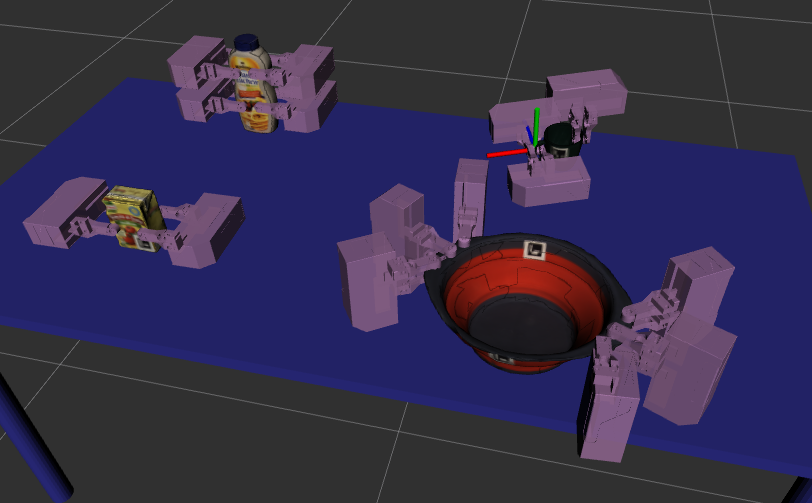
\includegraphics[width=0.6\linewidth, angle=0]{multiple_objects.png}
	\vspace{-10pt}
	\caption{Example of objects with predefined grasping poses}
	\vspace{-15pt}
	\label{fig:obj_grasp_pose}
\end{figure}

The proposed solution to this grasping problem includes generating a data base of objects with predefined grasping poses (GP) (figure \ref{fig:obj_grasp_pose}) and a perception system that detects the stored objects and shows the possible GP and it's position with respect to the robot.

The robot will have to decide which GP is better for grasping a specified object given a initial configuration. Then, a optimization controller (section \ref{sec:motion_controller}) will generate several possible trajectories, evaluate them and send the best one to the robot.


% Why is this an interesting problem? If solved, what is then possible?
% What is your approach to solving this problem?

\section{Contributions}
Data, software, algorithms, designs, etc... made by me
If the problem was solved, how was that done?

\section{Structure of the thesis}

%\begin{figure}[H]
%	\centering
%	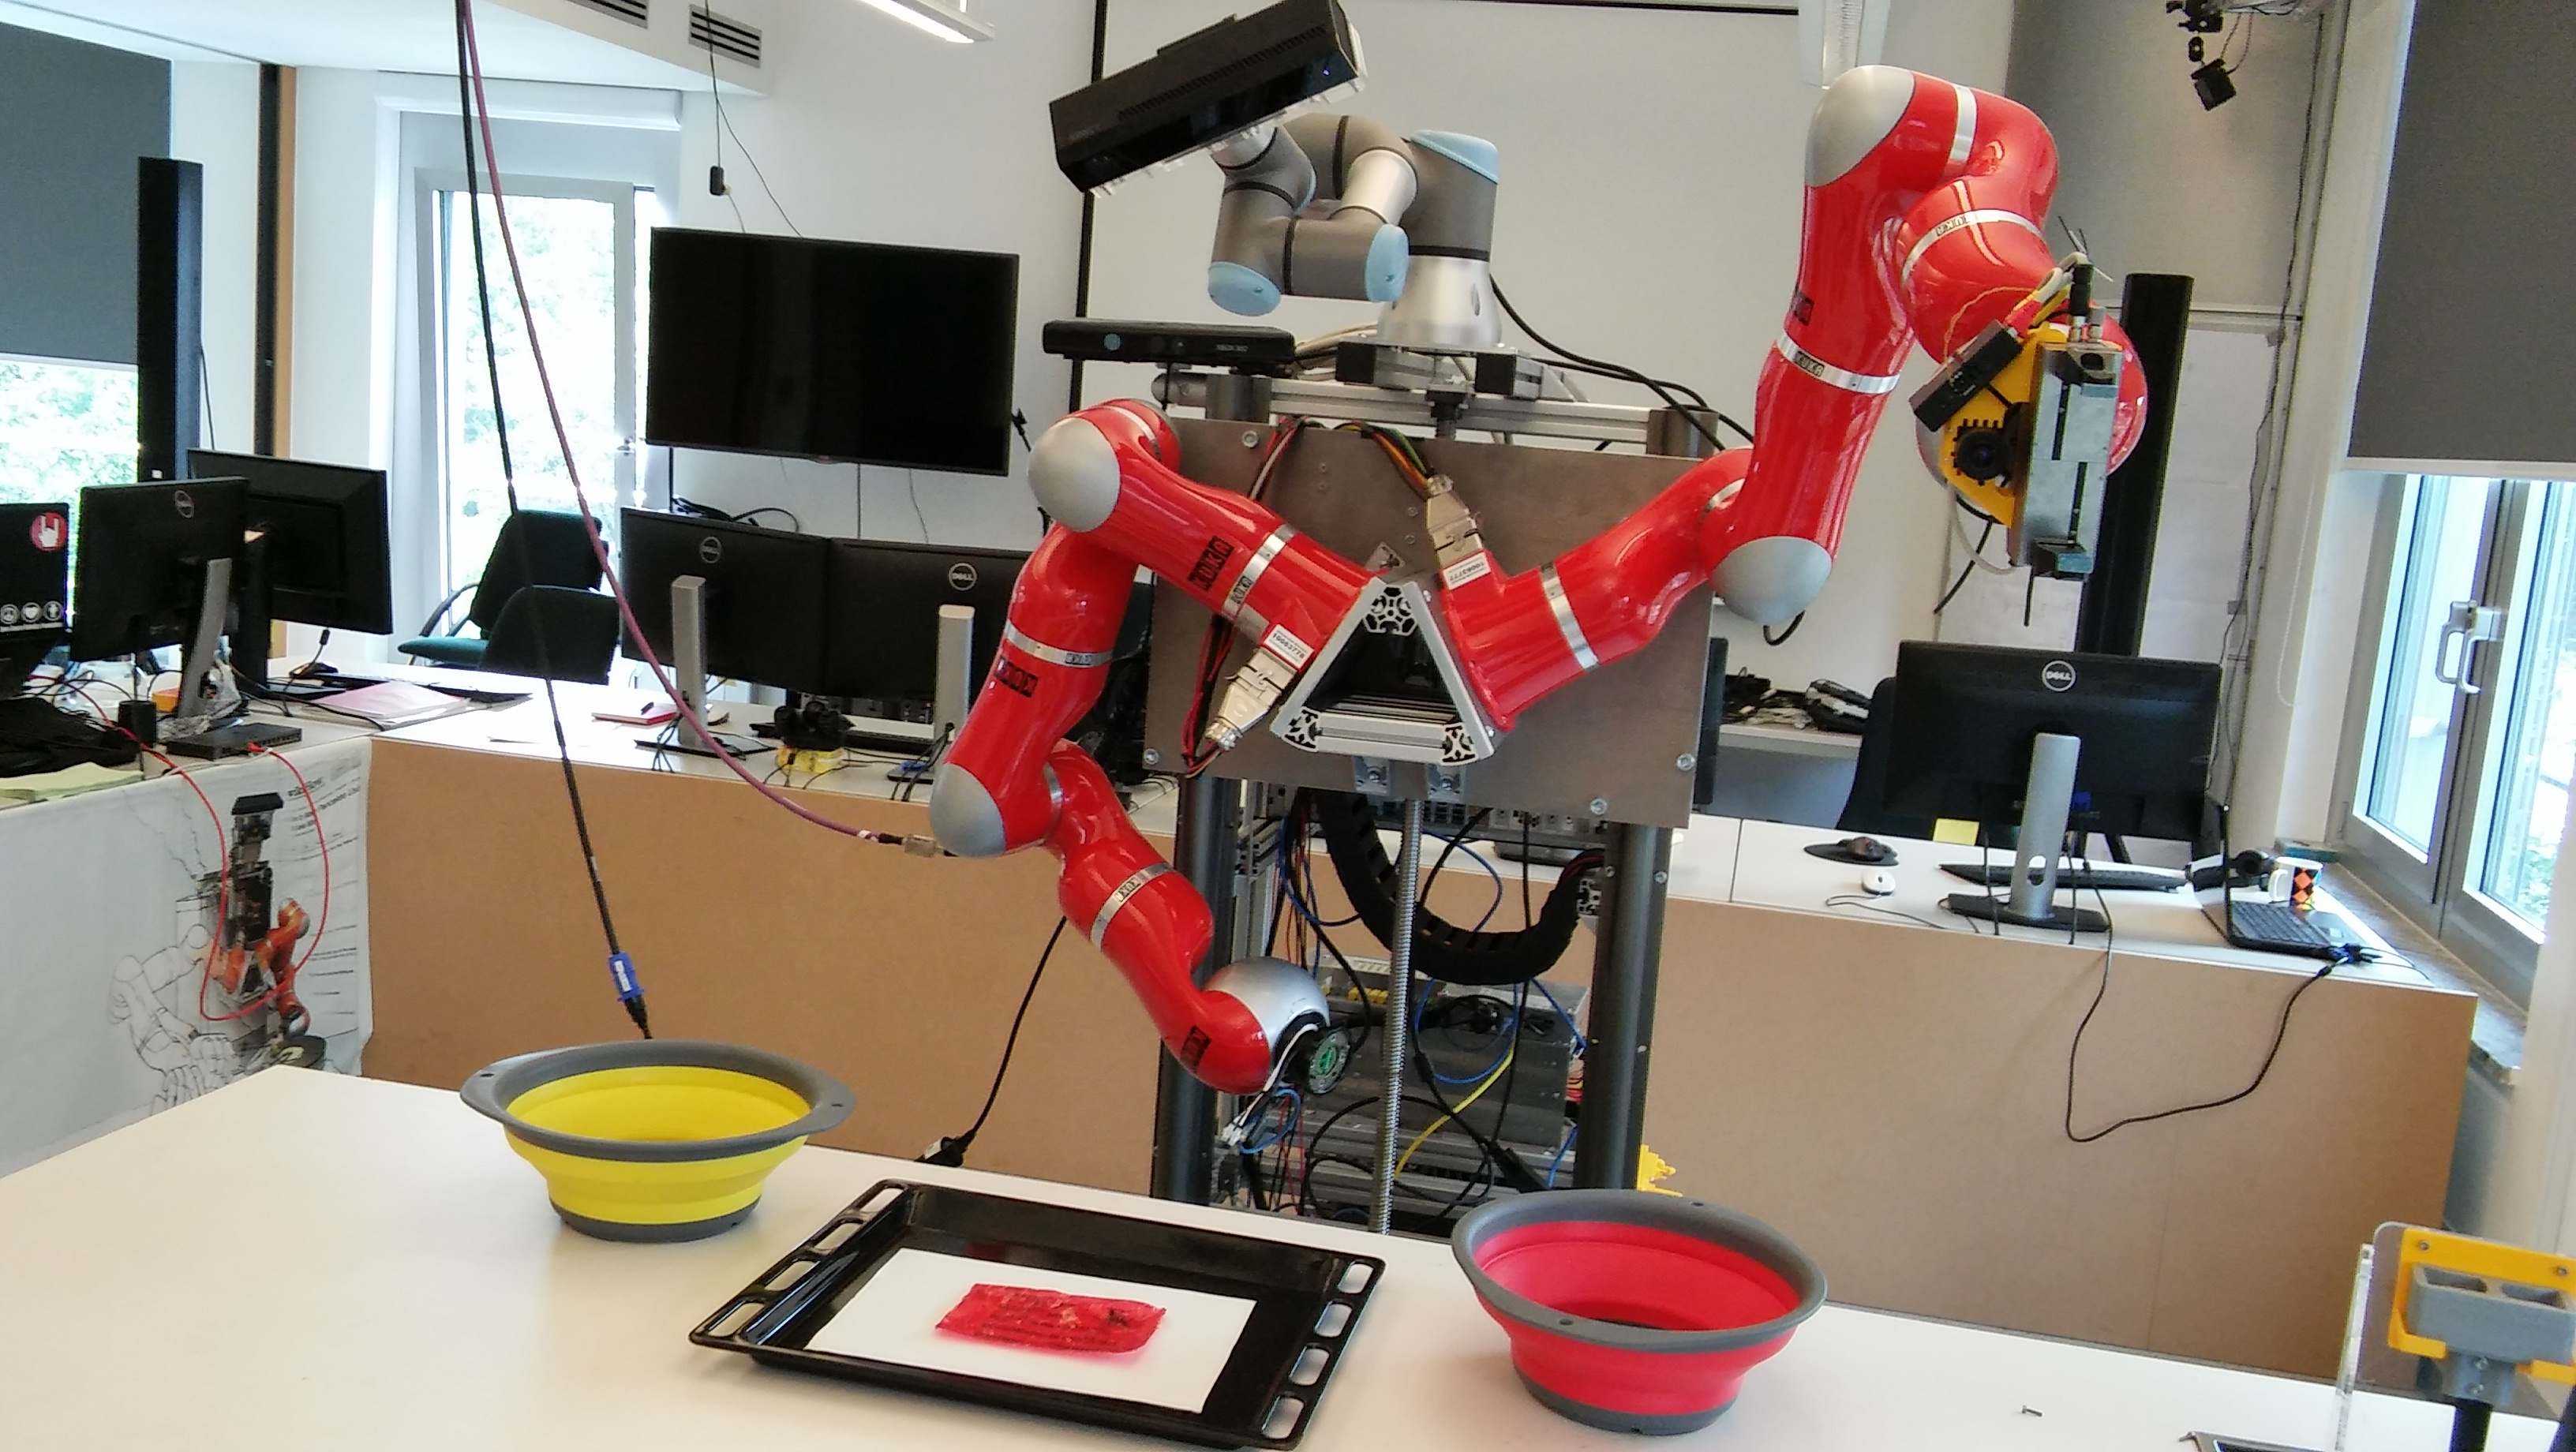
\includegraphics[width=0.6\linewidth, angle=0]{boxy/Boxy3.jpg}
%	\vspace{-10pt}
%	\caption{Boxy Robot}
%	\vspace{-15pt}
%	\label{fig:boxy}
%\end{figure}

